\textbf{Ejemplo 2}\\
Un proyecto requiere de una inversión inicial de 100.000 COP y se cree que generará unos i
ngresos de 65.000 COP al final del primer año y de 75.000 COP al final del segundo año. 
Evaluar el proyecto para el inversionista A cuya tasa es del 20\% pav, y para el inversionista B cuya tasa es del 40\% pav.\\


%%%%%%%%%%%%%%%%%%% EJERCICIO 2 %%%%%%

%\newpage %USAR SOLO SI EL SOLUCION QUEDA SOLO Y ES NECESARIO BAJARLO A LA SIGUIENTE PAGINA
\textbf{Solución.}\\
%La tabla ira centrada
\begin{center}
	\renewcommand{\arraystretch}{1.5}% Margenes de las celdas
	%Creacion de la cuadricula de 3 columnas \end{flushleft}
	\begin{longtable}[H]{|C{0.3\linewidth}|C{0.3\linewidth}|C{0.3\linewidth}|}
		%Creamos una linea horizontal
		\hline
        %%%%% INICIO FLUJO DE CAJA
		\rowcolor[HTML]{FFB183}
		\multicolumn{3}{|c|}{\cellcolor[HTML]{FFB183}\textbf{1. Asignación periodo focal}}   \\ \hline
		\multicolumn{3}{|c|} {$ff = 0 pav$} \\ \hline
		%%%%%%%%%% FIN TITULO
		%%%%%%%%%% INICIO TITULO
		%Lo que se hace aqui es mezclar las 3 columnas en una sola
		\multicolumn{3}{|c|}{\cellcolor[HTML]{FFB183}\textbf{2. Declaración de variables}}   \\ \hline
		%%%%%%%%%% FIN TITULO
		%%%%%%%%%% INICIO DE MATEMATICAS
		%Cada & hace referencia al paso de la siguiente columna
		$n_{0} = 0 pav$   & $n_{1} = 1 pav$ & $n_{2} =  2 pav$\\ \hline
		\multicolumn{3}{|c|}{$i_{A} = TIO_{A} = 20\% pav \equiv 0.2 pav$} \\
		\multicolumn{3}{|c|}{$i_{B} = TIO_{B} = 40\% pav \equiv 0.4 pav$} \\ \hline
		%%%%%%%%%% FIN DE MATEMATICAS
		%%%%% FIN DECLARACION DE VARIABLES


  	%%%%% INICIO DECLARACION FORMULAS
  
		%%%%%%%%%%% INICIO TITULO
		\rowcolor[HTML]{FFB183}
		\multicolumn{3}{|c|}{\cellcolor[HTML]{FFB183}\textbf{3. Diagrama de flujo de caja}} \\ \hline
		%Mezclamos 3 columnas y ponermos el dibujo
		%%%%%%%%%%%%% INSERCION DE LA IMAGEN
		%Deberan descargar las imagenes respectivas del drive y pegarlas en la carpeta
		%n_capitulo/img/ejemplos/1/capitulo1ejemplo1.pdf  (el /1/ es el numero del ejemplo)
		\multicolumn{3}{|c|}{ 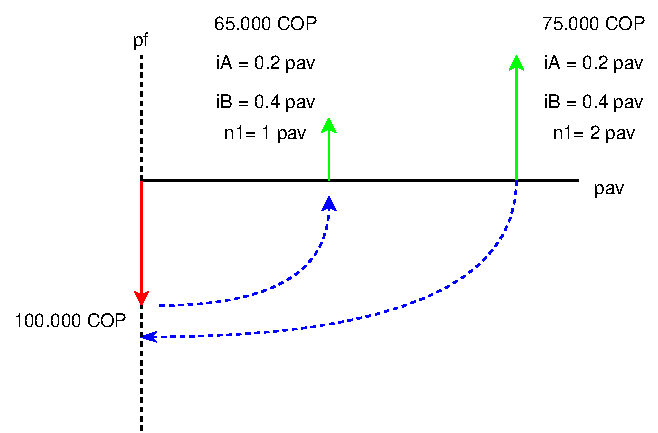
\includegraphics[trim=-5 -5 -5 -5 , scale=1.0, width=300px, height=250px]{9_Capitulo/ejemplos/2/Capitulo9Ejercicio2.pdf} }   \\ \hline
		%%%%%%%%%%%%% FIN INSERCION DE IMAGEN
		%%%%%FIN FLUJO DE CAJA



		%%%%% INICIO DECLARACION FORMULAS
		%%%%%%%%%%% INICIO TITULO
		\rowcolor[HTML]{FFB183}
		\multicolumn{3}{|c|}{\cellcolor[HTML]{FFB183}\textbf{4. Declaración de fórmulas}}    \\ \hline
		%%%%%%%%%%% FIN TITULO
		%%%%%%%%%%% INICIO MATEMATICAS
		\multicolumn{3}{|c|}{$\sum F_{n}(1+i)^{-n} $\hspace{0.3cm} \textit{Valor presente neto}} \\ \hline
		%%%%%%%%%% FIN MATEMATICAS
		%%%%%% INICIO DESARROLLO MATEMATICO
		\rowcolor[HTML]{FFB183}
		%%%%%%%%%%INICIO TITULO
		\multicolumn{3}{|c|}{\cellcolor[HTML]{FFB183}\textbf{5. Desarrollo matemático}}       \\ \hline
		%%%%%%%%%% FIN TITULO
		%%%%%%%%%% INICIO MATEMATICAS
		\multicolumn{3}{|c|}{$VPN_{A} = -100000 + 65000(1+0.2)^{-1} + 75000(1+0.2)^{-2}$} \\
		\multicolumn{3}{|c|}{$VPN_{A} = 6000.25$} \\
		\multicolumn{3}{|c|}{$VPN_{B} = -100000 - 65000(1+0.4)^{-1} + 75000(1+0.4)^{-2}$} \\
		\multicolumn{3}{|c|}{$VPN_{B} = 15000.31$} \\ \hline

		%%%%%%%%%% FIN MATEMATICAS
		%%%%%% FIN DESARROLLO MATEMATICO
		%%%%%% INICIO RESPUESTA
		\rowcolor[HTML]{FFB183}
		%%%%%%%%%%INICIO TITULO
		\multicolumn{3}{|c|}{\cellcolor[HTML]{FFB183}\textbf{6. Respuesta}}   \\ \hline
		%%%%%%%%%% FIN TITULO
		%%%%%%%%%% INICIO RESPUESTA MATEMATICA
		\multicolumn{3}{|c|}{Para el inversionista A el proyecto puede ser ejecutado, en cambio} \\ 
		\multicolumn{3}{|c|}{para el inversionista B no puede ser ejecutado.}  \\ \hline
		%%%%%%%%%% FIN MATEMATICAS
		%%%%%% FIN RESPUESTA
	\end{longtable}
	%Se crean dos lineas en blanco para que no quede el siguiente texto tan pegado
	%\newline \newline %USARLO SI CREES QUE ES NECESARIO
\end{center}
%%%%%%%%%%%%%%%%%%%%%%%%%%FIN EJERCICIO 2 %%%%%%%%%%%%%%%%%%%%%%%%%%%
